\begin{figure}[t]
\centering
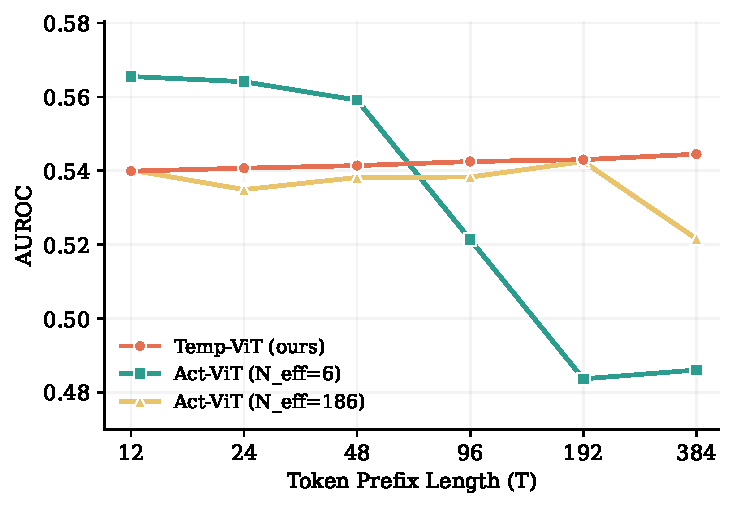
\includegraphics[width=0.95\linewidth]{figs/fig_perf_by_length.pdf}
\caption{Per-token AUROC on the LongFact prefix-truncation test as the
generated-token prefix length $T$ fed to each model grows. ACT-ViT
with its default short pooled token axis (\emph{Act-ViT, N\textsubscript{eff}=6})
peaks at short prefixes but collapses past $T = 48$ and falls below
chance for $T \in \{192, 384\}$ as the pooling compresses an
increasing number of token positions into the same fixed-size image.
Raising the pooled axis (\emph{Act-ViT, N\textsubscript{eff}=186})
partially rescues long prefixes but does not match Temp-ViT's flat
profile, which is per-token by construction. This illustrates the
long-form weakness of activation-tensor methods that pool the token
axis into a fixed-size representation.}
\label{fig:perf_by_length}
\end{figure}
